\documentclass[xcolor=x11names,compress]{beamer}
\usepackage[utf8]{inputenc}
\usepackage[spanish]{babel}
\usepackage{hyperref}
\hypersetup{colorlinks=true,linkcolor=black}
\usepackage{colortbl}
\usepackage{xcolor}
\usepackage{multirow}
\usepackage{fancyhdr}
\usepackage{graphicx}
\usepackage{framed}
\usepackage[version=0.96]{pgf}


\definecolor{shadecolor}{RGB}{243,243,243}
\renewcommand{\figurename}{Figura}

\newtheoremstyle{cuadrado}% name
  {1pt}%      Space above
  {8pt}%      Space below
  {\itshape}%         Body font
  {}%         Indent amount (empty = no indent, \parindent = para indent)
  {\itshape}% Thm head font
  {}%        Punctuation after thm head
  {0em}%     Space after thm head: " " = normal interword space;
        %       \newline = linebreak
  {}%         Thm head spec (can be left empty, meaning `normal')

\theoremstyle{cuadrado}
\newtheorem*{teo}{}


\newcommand{\slidesettitulo}{\textcolor{black}{Asistente de diseño de interfaz de control, seguimiento y sharing de
robots en tiempo real}}
\newcommand{\shorttitulo}{RobotUI}
\newcommand{\email}{\vspace*{.1in}{
\includegraphics[width=5.5cm]{logotipo.png}}}
\newcommand{\web}{}
\newcommand{\institucion}{Universidad de Cádiz  \\ Escuela Superior de Ingeniería}
\newcommand{\authornombre}{Manuel López Urbina}
\vspace*{2ex} 
\newcommand{\tutor}{Arturo Morgado Estévez}
\newenvironment{fondo}{\begin{teo}}{\end{teo}}


\definecolor{darkgray}{RGB}{237,236,236}
\definecolor{azuladwys}{RGB}{157,189,219}
\definecolor{azuladwys_version}{RGB}{174,208,239}
\definecolor{plata}{RGB}{145,143,144}


\usetheme{Ilmenau}

\setbeamertemplate{footline}{
\begin{tiny}
\setbeamercolor{foot1}{fg=black!70,bg=gray!10}
\setbeamercolor{foot2}{fg=gray,bg=gray!15}
\setbeamercolor{foot3}{fg=gray,bg=gray!10}
\setbeamercolor{foot4}{fg=black!70,bg=gray!20}
\setbeamercolor{foot5}{fg=gray,bg=gray!15}
\setbeamercolor{foot6}{fg=black,bg=gray!20}

%\setbeamercolor{foot1}{fg=azuladwys_version,bg=azuladwys_version}
%\setbeamercolor{foot2}{fg=azuladwys,bg=azuladwys}
%\setbeamercolor{foot3}{fg=azuladwys_version,bg=azuladwys_version}
%\setbeamercolor{foot4}{fg=azuladwys,bg=azuladwys}
%\setbeamercolor{foot5}{fg=azuladwys,bg=azuladwys}
%\setbeamercolor{foot6}{fg=black,bg=gray!20}

% taken from theme infolines and adapted
  \leavevmode%
  \hbox{%
  \begin{beamercolorbox}[wd=.35\paperwidth,ht=2.25ex,dp=1ex,center]{foot1}%
  %\fontsize{5}{5}\selectfont
  \shorttitulo
  \end{beamercolorbox}%
  \begin{beamercolorbox}[wd=.1\paperwidth,ht=2.25ex,dp=1ex,center]{foot2}
  \end{beamercolorbox}%
    \begin{beamercolorbox}[wd=.05\paperwidth,ht=2.25ex,dp=1ex,center]{foot3}
  \end{beamercolorbox}%
    \begin{beamercolorbox}[wd=.25\paperwidth,ht=2.25ex,dp=1ex,center]{foot4}%
  %\fontsize{5}{5}\selectfont
  \web
  \end{beamercolorbox}%
  \begin{beamercolorbox}[wd=.05\paperwidth,ht=2.25ex,dp=1ex,center]{foot5}
  \end{beamercolorbox}%
  \begin{beamercolorbox}[wd=.2\paperwidth,ht=2.25ex,dp=1ex,right]{foot6}%
	\insertframenumber{} / \inserttotalframenumber \hspace*{2ex} 
  \end{beamercolorbox}}%
  \vskip0pt%
\end{tiny}
\vskip10pt
}


%\setbeamertemplate{footline}{}
\setbeamertemplate{navigation symbols}{} %Elimina los iconos que permiten la navegación en el documento

\usecolortheme[named=darkgray]{structure}
\usefonttheme{professionalfonts}
\useoutertheme{miniframes}

\title{\slidesettitulo}
\author{\authornombre \\ \email \\ Director: \tutor}
\institute{\institucion}
\date{ }
\setcounter{subsection}{0}




\begin{document}
\scriptsize{

\frame{\titlepage

}

\section{Índice}
\frame{\frametitle{\textcolor{black}{Índice}}
  \textcolor{black}{\tableofcontents}
}

\section{Planificación}

\frame{\frametitle{\textcolor{black}{Tareas}}

\begin{figure}[H]
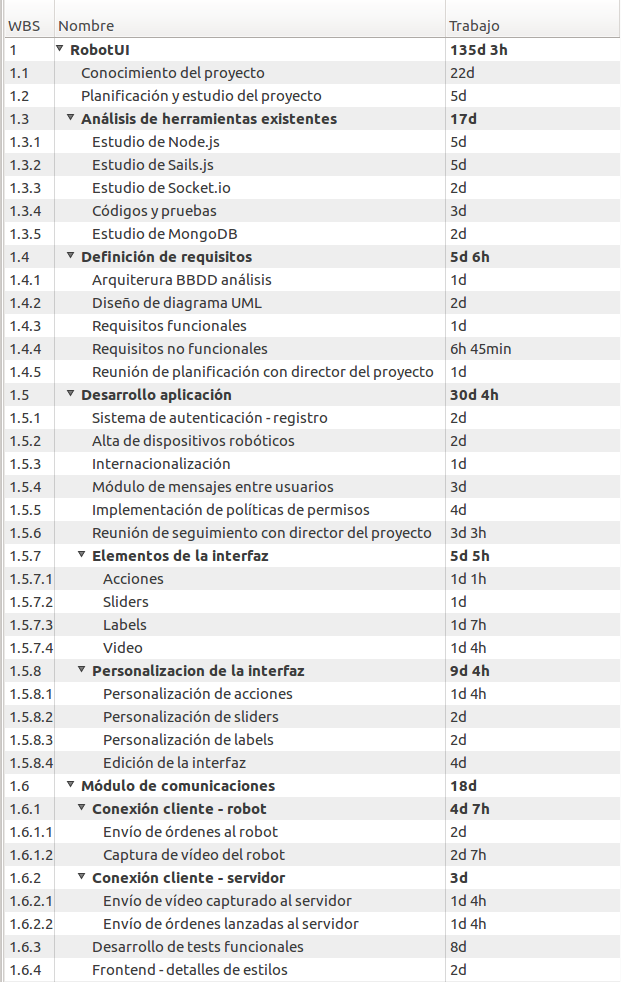
\includegraphics[width=6.5cm]{descomposicion_tareas01.png}
\end{figure}

}

\frame{\frametitle{\textcolor{black}{Diagrama de Gantt}}

\begin{figure}[H]
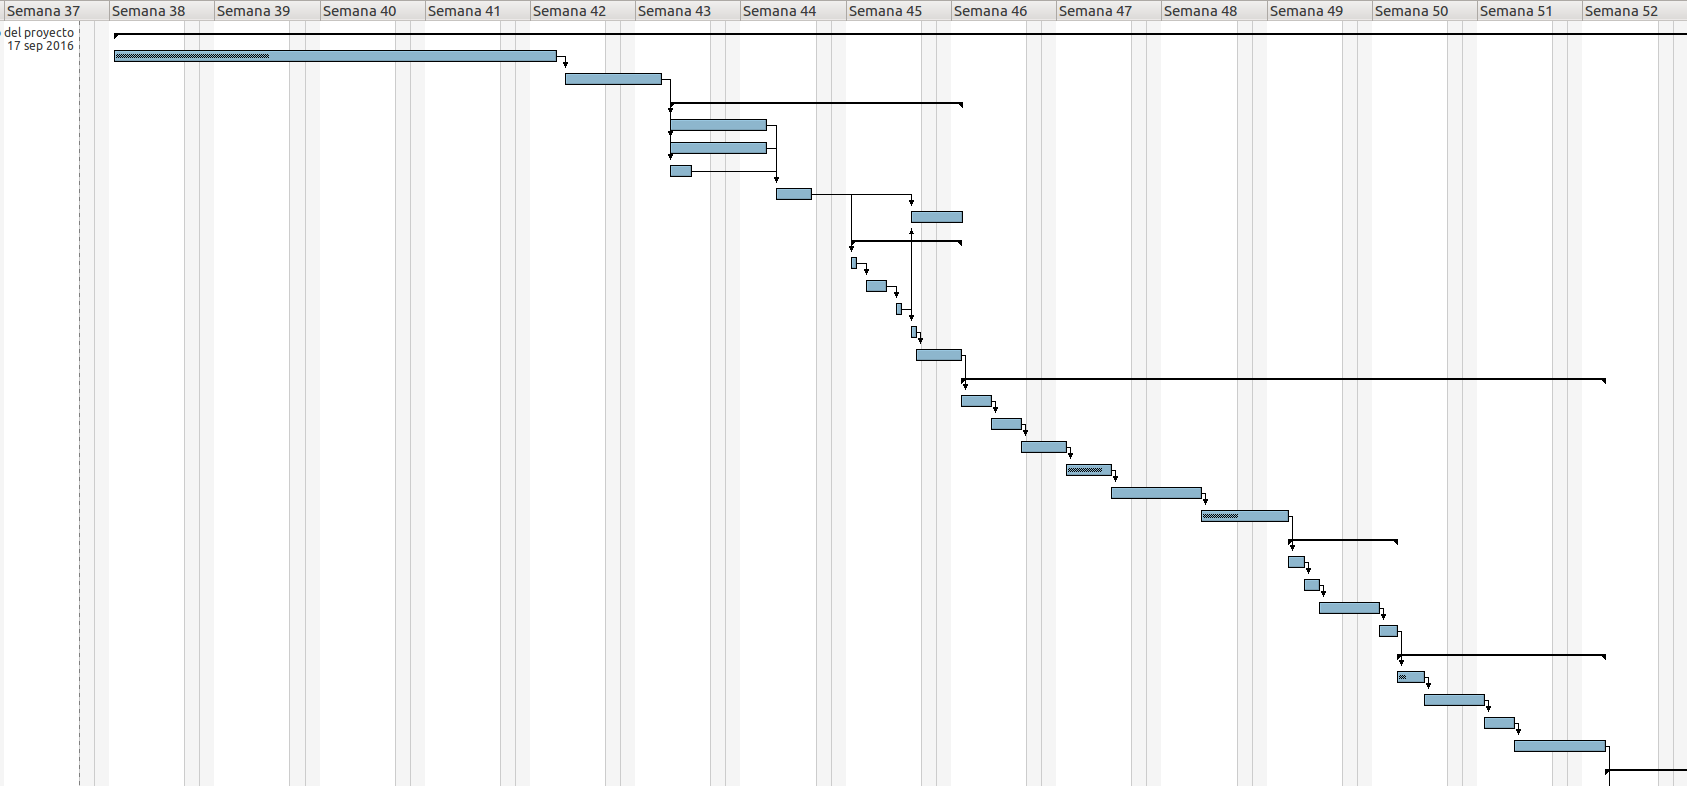
\includegraphics[width=4.4cm]{gantt01.png}
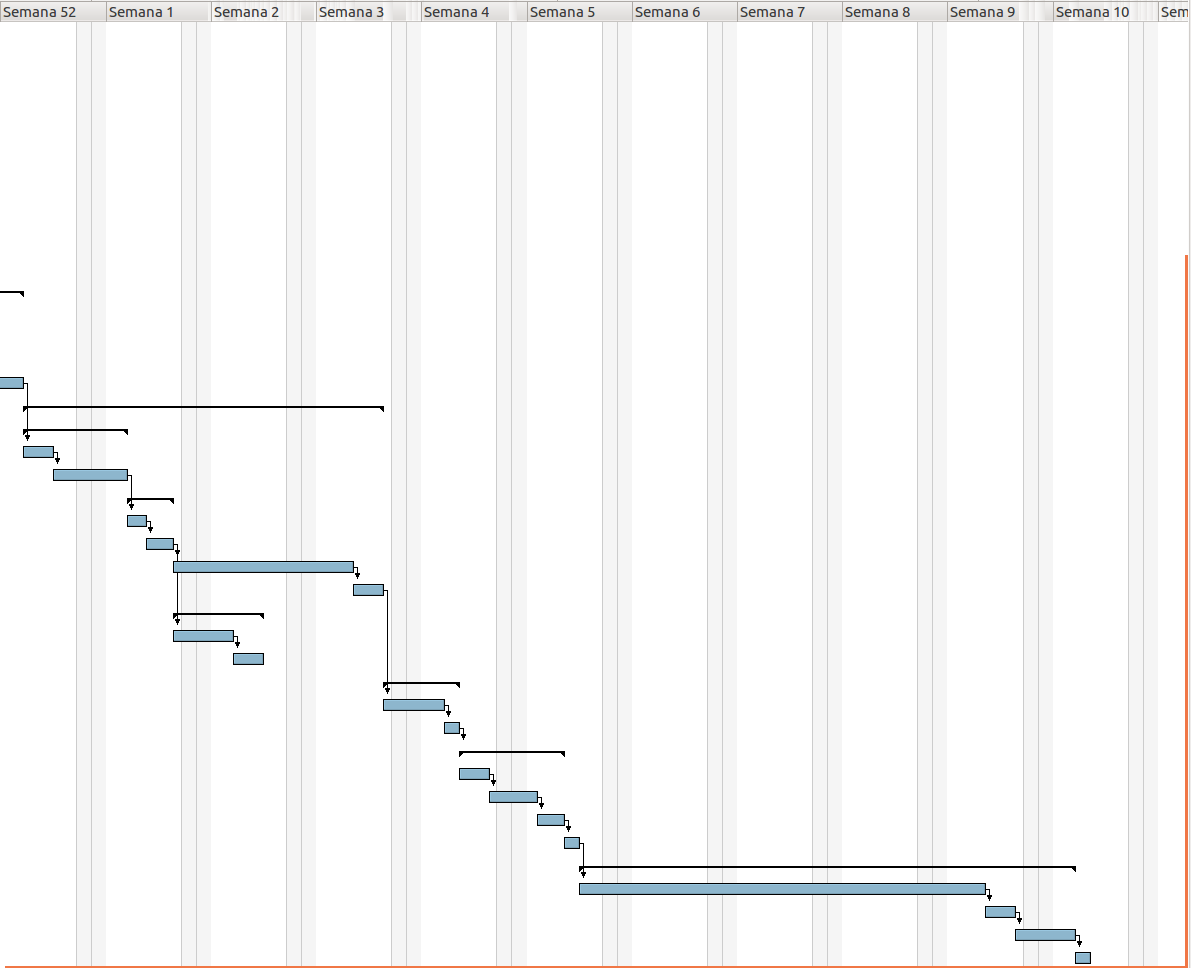
\includegraphics[width=4.4cm]{gantt02.png}
\end{figure}

}




\section{Conclusiones}

\frame{\frametitle{\textcolor{black}{Objetivos logrados}}
  Durante la realización del proyecto \emph{OpenTSR: Vehículo reconocedor de señales de tráfico} como trabajo de fin de carrera, he conseguido profundizar mi conocimiento en los siguientes campos:

  \begin{itemize}
  \item La elaboración de un vehículo de pruebas haciendo uso de una Raspberry Pi 3 Model B.
  \item Aprendizaje a la utilización del framework Sails.js.
  \item Trabajo con eventos en tiempo real mediante el empleo de WebSockets, de la cual se han adquirido conocimientos que no dudo que me serán de utilidad para futuros proyectos y desarrollos.
  \item Empleo de una base de datos no relacional como Mongo DB.
  \item Transmisión de gran cantidad de datos entre cliente servidor y servidor cliente. Streaming de vídeo y emisión de comandos entre otros datos.
  \end{itemize}
}


\end{document}
